\documentclass[11pt, letterpaper]{article}

% ABNT %
\usepackage[brazil]{babel}
\usepackage[utf8]{inputenc}
\usepackage[margin=1in]{geometry}
% FIGURAS %
\usepackage{graphicx}
\usepackage{fancyhdr}
\usepackage{setspace}
\usepackage{subfig}
\usepackage{float}
%
\usepackage{placeins}
\renewcommand{\contentsname}{Sumário}
%------------------------------------------------------
\begin{document}
\begin{titlepage}
\thispagestyle{empty}
\parbox{1.5cm}{
\includegraphics[scale=0.25]{logo_uerj_cinza.png}}
\vspace*{-0.8cm}{\hspace*{1.5cm} \Large{\textbf{Universidade do Estado do Rio de Janeiro}\\
\hspace*{5.3cm}}}
\Large{Departamento de Física Teórica} \\

\vspace{5cm}
\hspace{4.5cm} \Large{\textbf{Estimativas de $\pi$ com incertezas}}
\vspace{8cm}

\begin{flushright}
Aluno: José Gonçalves Chaves Junior \\
M:202020477411\\
Curso: Física 
\end{flushright}

\end{titlepage}
%-----------------------------------------------------------------
\tableofcontents

\newpage
\listoftables
\newpage
%-----------------------------------------------------------------
\section{Introdução}
%-----------------------------------------------------------------
O número pi, representa o valor da razão entre o perímetro (p) e o diâmetro (d) de uma circunferência qualquer.
\begin{equation}
\pi = \frac{p}{d}
\end{equation}
Desde a Antiguidade, com os egípcios e os babilônios, o número pi já era estudado: escribas egípcios já continham um valor aproximado para a constante matemática mais antiga do mundo.


Com o passar dos anos, o número foi sendo ainda mais estudado, chegando até Ptolomeu, que por volta do século III d.C, calculou pi a partir de um polígono inscrito em uma circunferência. Com isso, achou pi como um valor próximo de 3,1416.


Na contemporaneidade, o número se mostra extremamente importante: desde os primeiros relógios de pêndulo, até ao cálculo de volume de combustível usado por aviões.
%----------------------------------------------------------------
\section{Objetivo}
%----------------------------------------------------------------

Neste Experimento, o objetivo é estimar o valor de pi através de dois métodos:

a) medindo uma panela (objeto fabricado com seção transversal considerada circular);


b) com uma circunferência desenhada pelo próprio aluno;

e, após, verificar se os resultados são compatíveis ou não com o valor de \pi .

%----------------------------------------------------------------
\section{Procedimento Experimental}
%----------------------------------------------------------------
Para realizar as medições, foi usado:
\begin{enumerate}
\item Uma linha de costura (100,00 $\pm$ 0,05 cm);
\item Uma folha A4 (210mm x 297mm);
\item Superfície de uma mesa (5m x 1,4 m);
\item Caneta Esferográfica de cor Azul (15cm x 0,5cm x 0,5 cm);
\item Fita métrica de 30 cm; \\
Para estimar os valores de comprimento e diâmetro das circunferências, mediu-se seus valores 10 vezes, com a finalidade de chegar a um valor mais coerente.
\newpage
%----------------------------------------------------------------
\section{Análise dos Dados Coletados}
%----------------------------------------------------------------
%medicoes feitas na circunferencia de papel
\FloatBarrier
\begin{table}[!ht]
\caption{Medições realizadas da circunferência feita no papel}
\centering
\begin{tabular}{|l|l|}
\hline
Comprimento (cm) & Diâmetro (cm)\\
\hline
45.40 & 15.10\\
\hline
46.40 & 15.12\\
\hline
46.38 & 15.00\\
\hline
46.50 & 15.20\\
\hline
46.30 & 15.11\\
\hline
46.29 & 15.09\\
\hline
46.31 & 15.09\\
\hline
46.30 & 15.10\\
\hline
46.29 & 15.00\\
\hline
46.30 & 15.00\\
\hline
\end{tabular}
\end{table}
\FloatBarrier
%medicoes feitas na circunferencia da panela
\begin{table}[!ht]
\caption{Medições realizadas da circunferência na panela}
\centering
\begin{tabular}{|l|l|}
\hline
 Comprimento (cm) & Diâmetro (cm)\\
\hline
66,52 & 21,50\\
\hline
66,65 & 21,49\\
\hline
66,80 & 21,53\\
\hline
66,72 & 21,53\\
\hline
66,73 & 21,50\\
\hline
66,68 & 21,50\\
\hline
66,63 & 21,50\\
\hline
66,75 & 21,38\\
\hline
66,73 & 21,49\\
\hline
66,72 & 21,50\\
\hline
\end{tabular}
\end{table}
\newpage
%-------------------------------------
\FloatBarrier
\begin{table}[!ht]
\caption{Dados da circunferência da Panela}
\centering
\begin{tabular}{|1|l|l|}
\hline
 - & Comprimento(cm) & Diâmetro (cm)\\
\hline
 Média & 66,69 & 21,50 \\
\hline
Desvio Padrão & 0,08  & 0,04 \\
\hline

\end{tabular}
\end{table}
\FloatBarrier
\begin{table}[!ht]
\caption{Dados da circunferência feita no papel}
\centering
\begin{tabular}{|1|l|l|}
\hline
- & Comprimento (cm) & Diâmetro (cm)\\
\hline
Média & 46,25 & 15,08 \\
\hline
  Desvio Padrão & 0,30 & 0,06\\
\hline
\end{tabular}
\end{table}
%----------------------------
%--------------------------
\FloatBarrier
\begin{table}[!ht]
\caption{Erro sistemático da circunferência no papel}
\centering
\begin{tabular}{|l|l|}
\hline
\sigma_{c}(cm) & \sigma_{d}(cm)\\
\hline
  0.096 & 0.020\\
\hline
\end{tabular}
\end{table}
%-------------------------
\FloatBarrier
\begin{table}[!ht]
\caption{Erro sistemático da circunferência na panela}
\centering
\begin{tabular}{|l|l|}
\hline
\sigma_{c}(cm) & \sigma_{d}(cm)\\
\hline
  0.50 & 0.50\\
\hline
\end{tabular}
\end{table}
\textit{\textbf{OBS:} Já contabilizado o erro sistemático em relação à linha de costura (0,05 cm).}
\subsection{Estimativas finais para o comprimento e o diâmetro}
%------------------------------------
\FloatBarrier
\begin{table}[!ht]
\caption{Circunferência feita na panela}
\centering
\begin{tabular}{|l|l|}
\hline
  Comprimento  &   Diâmetro \\
\hline
\textbf{66.69 ± 0.71 cm} &  \textbf{21.49 ± 0.71 cm} \\
\hline
\end{tabular}
\end{table}
\FloatBarrier
\begin{table}[!ht]
\caption{Circunferência feita no papel}
\centering
\begin{tabular}{|l|l|}
\hline
   Comprimento  &   Diâmetro \\
\hline
\textbf{46.25 ± 0.10 cm} & \textbf{15.08 ± 0.10 cm} \\
\hline
\end{tabular}
\end{table}
%-------------------------------------
\newpage
\section{Estimativas para \pi}
Para estimarmos o valor de pi através da circunferência no papel, utilizaremos o seguinte cálculo: 


\begin{equation}
\pi = \frac{c_{média}}{d_{média}} \pm \sigma_{papel}
\end{equation}
onde, 
\begin{equation}
\sigma_{papel} = \sqrt{{\sigma_{c}}^2/{media_{c}}^2 + {\sigma_{d}}^2/{media_{d}^2 }} = 0.007628 $ \\ cm 
\end{equation} \\
sendo assim, chegaremos à: 
\label{eq.1}
\begin{equation}
\Large*{\pi  = (3.07 \pm 0.01)} cm \\
\end{equation}
Analogamente para o valor de pi através da panela: \\
\begin{equation}
\pi = \frac{c_{média}}{d_{média}} \pm \sigma_{panela}
\end{equation}
onde, 
\begin{equation}
 \sigma_{panela} = \sqrt{{\sigma_{c}}^2/{media_{c}}^2 + {\sigma_{d}}^2/{media_{d}^2 }} =  0.075871 $ cm
\end{equation}
sendo assim, chegaremos à: \\
\label{eq.2}
\begin{equation} 
\Large*{\pi = (3.10 \pm 0.08)} cm 
\end{equation} 
\newpage
\section{Compatibilidade}
Com os nossos resultados, podemos verificar a compatibilidade destes, com o valor referência \pi = 3,141. 
% compatibilidade
\FloatBarrier
\begin{table}[!ht]
\caption{Dados para a compatibilidade com o valor referência}
\centering
\begin{tabular}{|1|1|1|}
\hline
- & Circunferência no Papel & Circunferência da Panela \\
\hline
Discrepância & 0,075 cm & 0,038 cm  \\
\hline
Erro Relativo & 0,0024 & 0,0244 \\
\hline
Erro Percentual & 0,24  & 2,44 \\
\hline 
\end{tabular}
\end{table}
%---------------

\begin{figure}[!htbp]
\centering
\begin{tabular}{11}
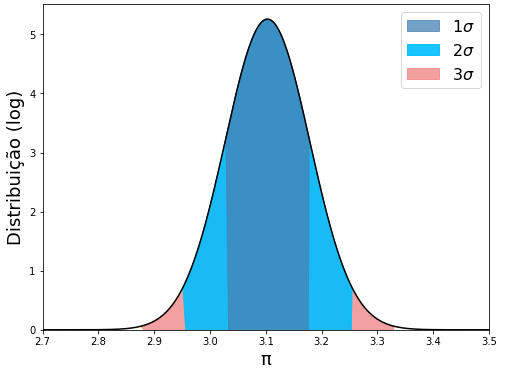
\includegraphics[width=0.4959\textwidth]{dis_pan.png} &
 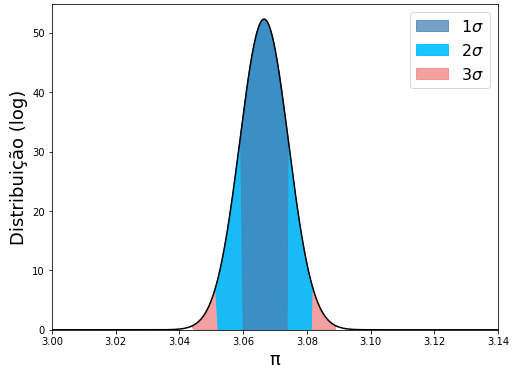
\includegraphics[width=0.5\textwidth]{dis_papel.png}
 \\
 (a) Panela & (b) Papel
\end{tabular}
\caption{Distribuição Gaussiana do valor de $\pi$ encontrado.}
\end{figure}
\newpage
\section{Conclusão}
Podemos perceber que, além dos valores encontrados nas equações 4 e 7, os gráficos de distribuição apontam para um intervalo mais satisfatório em relação à medição de $\pi$ através da panela que no papel. \\
Além disso, pela discrepância, observamos que o valor de $\pi$ encontrado quando medido pela panela se torna compatível com o valor referência, pois $ 2\sigma_{panela} = 0.151743 $ e portanto, com a discrepância apresentada, o valor está num intervalo menor que $2\sigma_{panela}$. Por outro lado, por mais que o erro da circunferência no papel seja consideravelmente menor que da panela, o valor apresentado pela circunferência no papel não se encontra próximo do valor referência, com um valor bem discrepante do referente.

\subsection{Respostas}
\textbf{1}-Por mais contraintuitivo possa parecer, medir um objeto maior aumentou a precisão do resultado (por mais que o resultado não pareça ser tão próximo do ideal). Então, essa questão depende de que forma e quais instrumentos usamos para medir o círculo. Portanto, fico com a resposta de medir um círculo maior. \\
\textbf{2}- Realizei 10 medições; Aumentou a acurácia do meu resultado. Por realizarmos várias medidas e depois realizarmos a média, contamos com a ajuda de um valor "mais próximo do ideal", e por isso, a realização de várias medições ajuda consideravelmente a achar o valor real. O cálculo das incertezas muda, pois o erro passa a depender da raiz da quantidade de medidas feitas.\\
\textbf{3}- Talvez mudaria o método de medição. Utilizar, por exemplo, uma medição à laser ou algum programa que conseguisse medir o comprimento da circunferência (como uma régua "dobrável"). Além disso, realizar mais medições, além das 10; querendo ou não, aumentaria a acurácia em relação à média de comprimento e diâmetro.\\
\textbf{4}- Da definição de objeto circular, precisamos do valor de $\pi$ para calcular "o quão próximo de um círculo" um objeto pode ser. Como $\pi$ é uma constante matemática, a realização desse experimento é uma boa aproximação de um experimento "ideal" para verificar o quão perfeitamente circular é um objeto.\\
\newpage
\section{Bibliografia}
 Ref. 1: https://www.educamaisbrasil.com.br/enem/matematica/numero-pi ; \\
 Ref. 2: https://www.todamateria.com.br/numero-pi/ ; \\ 
 Ref. 3: \textit{“Estimativas e erros em experimentos de Física”}, coleção Comenius, 3a
 Edição. Ed UERJ. \\

\end{document}

